% =====================================================================
%  TA-PFC-E1 — Proyecto Fin de Curso, entrega 1
%  SGIRI Distribuido — Sistema de Gestión de Incidencias
%
%  Compilación (desde esta carpeta):
%      pdflatex main.tex
%      biber main
%      pdflatex main.tex
%      pdflatex main.tex
%
%  No usar minted ni rutas absolutas: el PDF debe regenerarse al clonar.
% =====================================================================
\documentclass[11pt,a4paper]{article}

\usepackage[utf8]{inputenc}
\usepackage[T1]{fontenc}
\usepackage{lmodern}
\usepackage[spanish,es-tabla]{babel}
\usepackage[margin=2.5cm]{geometry}
\usepackage{graphicx}
\usepackage{array}
\usepackage{booktabs}
\usepackage{tabularx}
\usepackage{longtable}
\usepackage{float}
\usepackage{xcolor}
\usepackage{caption}
\usepackage{csquotes}
\usepackage{microtype}
\usepackage[hidelinks]{hyperref}
\usepackage[backend=biber,style=ieee]{biblatex}

\addbibresource{referencias.bib}

\newcolumntype{Y}{>{\raggedright\arraybackslash}X}
\newcommand{\pendiente}[1]{\textcolor{red}{\textbf{[PENDIENTE: #1]}}}
\newcommand{\repo}{\url{https://github.com/Amendozab5/sgiri-distribuido}}

\captionsetup{font=small,labelfont=bf}
\setlength{\parindent}{0pt}
\setlength{\parskip}{6pt}

% Marcador de figura mientras no exista el archivo exportado
\setlength{\emergencystretch}{1.5em}
\newcommand{\pd}{\textcolor{red}{\textbf{?}}}

\newcommand{\figurapendiente}[1]{%
  \fbox{\parbox[c][4.5cm][c]{0.88\linewidth}{\centering\small\pendiente{#1}}}}

\begin{document}

% ---------------------------------------------------------------------
% Portada
% ---------------------------------------------------------------------
\hypersetup{pageanchor=false}
\begin{titlepage}
\centering
{\large\scshape Universidad Técnica Estatal de Quevedo\par}
\vspace{0.2cm}
{\normalsize \pendiente{facultad y carrera}\par}
\vspace{0.6cm}
{\normalsize Aplicaciones Distribuidas --- Séptimo nivel, paralelo B\par}
{\normalsize Periodo académico \pendiente{periodo}\par}
\vspace{1.8cm}
{\Huge\bfseries SGIRI Distribuido\par}
\vspace{0.5cm}
{\Large Sistema de Gestión de Incidencias para proveedores de servicios de internet\par}
\vspace{0.4cm}
{\large Proyecto Fin de Curso --- Entrega 1\par}
{\normalsize Definición, requisitos y arquitectura base del sistema distribuido\par}
\vspace{1.5cm}

{\small
\begin{tabularx}{\linewidth}{@{}l l Y@{}}
\toprule
\textbf{Integrante} & \textbf{Rol} & \textbf{Responsabilidad principal} \\
\midrule
Zambrano Yong Angel Daniel & Arquitecto y Documentación & C4, ADR, CAP/PACELC, integración del documento \\
Mendoza Bermello Angello Agustín & Líder de Desarrollo & Esqueleto funcional y comunicación entre servicios \\
Macías Vásquez César Abraham & Responsable de Calidad & Requisitos, riesgos, pruebas y coherencia \\
\bottomrule
\end{tabularx}}

\vspace{1.5cm}
{\normalsize Fecha de entrega: 29 de noviembre de 2026\par}
\vspace{0.3cm}
{\normalsize Repositorio: \repo\par}
\vspace{1.0cm}
{\small \pendiente{nombre del docente}\par}
\end{titlepage}
\hypersetup{pageanchor=true}

\pagenumbering{roman}
\tableofcontents
\clearpage

\pagenumbering{arabic}

% ---------------------------------------------------------------------
% Contenido (cada sección vive en su propio archivo para que cada
% integrante pueda trabajar y confirmar por separado)
% ---------------------------------------------------------------------
\section{Resumen ejecutivo}

\pendiente{Redactar entre 300 y 400 palabras. Contar al final con un script; el límite es parte del
requisito.}

% ---------------------------------------------------------------------
% Guía de redacción (borrar los comentarios al terminar):
%  1. Qué problema real resuelve el sistema y para qué organización
%     concreta (nombre o seudónimo autorizado en el acta), no "las empresas".
%  2. Quién lo usará: clientes, mesa de ayuda, técnicos de campo.
%  3. Cómo se resuelve hoy el problema y qué consecuencia medible tiene
%     (tiempo, costo, errores) según el acta de la entrevista.
%  4. Por qué la solución debe ser distribuida: dos razones ligadas
%     directamente a RNF-01 (disponibilidad) y RNF-02 (escalabilidad),
%     sin definiciones de manual.
%  5. Alcance del periodo: qué se construye en E1, E2, E3 y E4, y qué
%     queda explícitamente fuera.
% ---------------------------------------------------------------------

\section{Contexto y problema}

\subsection{Organización y usuarios}

\pendiente{Describir la organización real (o el grupo de usuarios) con los datos del acta:
nombre o seudónimo autorizado, actividad, tamaño, ubicación, horario de atención y volumen de
casos por semana. Si se usa seudónimo, indicarlo y explicar por qué.}

\subsection{Cómo se resuelve hoy}

\pendiente{Describir el proceso actual con sus herramientas reales (hoja de cálculo, WhatsApp,
cuaderno, sistema anterior), quién hace qué y en qué orden. Un párrafo por paso del proceso.}

\subsection{Consecuencias medibles de no resolverlo}

Cada cifra de esta tabla debe poder rastrearse hasta una frase del acta (anexo~\ref{anexo:acta}).

\begin{table}[H]
\centering
\caption{Consecuencias actuales del problema}
\label{tab:consecuencias}
\small
\begin{tabularx}{\linewidth}{@{}lYY@{}}
\toprule
Indicador & Valor actual & Fuente \\
\midrule
Tiempo medio de registro de una incidencia & \pendiente{cifra} & Acta, pregunta \pendiente{n} \\
Tiempo medio de asignación al técnico & \pendiente{cifra} & Acta, pregunta \pendiente{n} \\
Casos perdidos o duplicados por semana & \pendiente{cifra} & Acta, pregunta \pendiente{n} \\
Incidencias que vencen el SLA sin aviso & \pendiente{cifra} & Acta, pregunta \pendiente{n} \\
Costo estimado por hora de servicio detenido & \pendiente{cifra} & Acta, pregunta \pendiente{n} \\
\bottomrule
\end{tabularx}
\end{table}

\subsection{Interesados y expectativas}

\begin{table}[H]
\centering
\caption{Interesados del sistema y lo que esperan}
\label{tab:stakeholders}
\small
\begin{tabularx}{\linewidth}{@{}lYY@{}}
\toprule
Interesado & Qué espera del sistema & Cómo se comprueba \\
\midrule
Cliente final & Saber en qué va su caso sin llamar & Consulta de estado con número de ticket \\
Agente de mesa de ayuda & Registrar y clasificar rápido, sin duplicar & Formulario de alta en menos de 60 s \\
Técnico de campo & Ver su cola y actualizar el estado desde el celular & Interfaz adaptable y actualización sin conexión estable \\
Responsable de operaciones & Cumplir el SLA y ver la carga por técnico & Reporte de cumplimiento y tablero \\
Gerencia & Reducir el costo de atención & Indicador mensual de costo por caso \\
\bottomrule
\end{tabularx}
\end{table}

\subsection{Alcance del periodo}

\begin{table}[H]
\centering
\caption{Alcance por entrega}
\small
\begin{tabularx}{\linewidth}{@{}lY@{}}
\toprule
Entrega & Alcance comprometido \\
\midrule
E1 & Definición, requisitos, arquitectura C4, ADR, CAP/PACELC y esqueleto de dos servicios \\
E2 & Microservicios completos, API documentada y despliegue en contenedores \\
E3 & Base de datos distribuida y procesamiento de datos del SLA \\
E4 & Sistema final en capas, pruebas, calidad y defensa \\
\midrule
Fuera del alcance & \pendiente{facturación, aplicación móvil nativa, integración con el sistema del proveedor de red} \\
\bottomrule
\end{tabularx}
\end{table}

\section{Objetivos}

\subsection{Objetivo general}

Construir el SGIRI como un sistema distribuido que permita a un proveedor de internet registrar
cualquier incidencia técnica que reporten sus clientes y asignarla a un técnico especializado en
ese tipo de problema, de modo que una falla en una parte del sistema no detenga el registro ni la
atención de las incidencias.

\subsection{Objetivos específicos e indicadores}

\begin{table}[H]
\centering
\caption{Objetivos específicos y su indicador de cumplimiento}
\label{tab:objetivos}
\small
\begin{tabularx}{\linewidth}{@{}clY@{}}
\toprule
\# & Objetivo específico & Indicador con que se comprueba \\
\midrule
OE1 & Diseñar la arquitectura y comunicar dos servicios (E1)
& Los servicios de incidencias y técnicos responden por REST y devuelven 503 cuando el otro está
apagado; se comprueba con capturas el 29/11/2026 \\
OE2 & Agregar el API Gateway, las notificaciones con RabbitMQ y el despliegue con Docker Compose (E2)
& El sistema arranca con un solo \texttt{docker compose up} y las pruebas de humo pasan en la
semana 9 \\
OE3 & Probar la tolerancia a fallos y la carga (E3)
& Con 200 usuarios simultáneos, el 95\,\% de las consultas responde en menos de 300~ms (RNF-03 y
RNF-04), medido en la semana 13 \\
OE4 & Entregar el sistema completo con todos los requisitos funcionales (E4)
& Los 11 requisitos funcionales pasan sus criterios de aceptación y la disponibilidad medida
llega al 99,5\,\% (RNF-01) en la semana 17 \\
\bottomrule
\end{tabularx}
\end{table}

\section{Trabajos relacionados}

Se comparan al menos tres sistemas o estudios publicados que resuelven un problema equivalente
(gestión de incidencias, mesas de ayuda o sistemas distribuidos de atención). De cada uno se
indica qué se toma y en qué se diferencia el proyecto.

\begin{table}[H]
\centering
\caption{Comparación con trabajos relacionados}
\label{tab:relacionados}
\small
\begin{tabularx}{\linewidth}{@{}clYYY@{}}
\toprule
\# & Obra & Qué resuelve & Qué tomamos & En qué nos diferenciamos \\
\midrule
1 & Li et al. (2022)~\cite{li2022incident}
  & Detección proactiva de incidentes y generación automatizada de tickets ante degradación de
    rendimiento en servicios en la nube a gran escala.
  & Desacoplar el registro inicial del ticket del procesamiento de adjuntos y notificaciones para
    garantizar persistencia inmediata sin bloqueo.
  & Li et al. gestionan incidentes internos de centros de datos y telemetría; SGIRI atiende clientes
    residenciales de ISP, coordinando visitas de técnicos en campo con SLA en horas. \\
\addlinespace
2 & Harsh et al. (2023)~\cite{harsh2023murphy}
  & Diagnóstico y aislamiento de degradaciones intermitentes de rendimiento correlacionando reportes
    en tickets de soporte con trazas distribuidas.
  & Propagación de identificadores de correlación (\texttt{X-Correlation-Id}) en cada petición para
    auditar la trazabilidad completa del ticket entre microservicios.
  & Murphy enfoca el diagnóstico automático de trazas RPC; SGIRI aborda el flujo operativo humano
    completo: asignación por carga, seguimiento móvil y validación de evidencias. \\
\addlinespace
3 & Li et al. (2023)~\cite{li2023identifying}
  & Identificación de cambios de versión o configuración causantes de incidencias reportadas por
    usuarios en sistemas de servicios en línea.
  & Validación estricta de precondiciones y máquina de estados en el límite de la API para rechazar
    transiciones erróneas antes de despachar tareas al personal.
  & Su estudio se centra en incidentes de código en SaaS; SGIRI atiende la logística de técnicos
    desplazados con conectividad móvil intermitente y gestión de cuadrillas locales. \\
\bottomrule
\end{tabularx}
\end{table}

\section{Requisitos}

\subsection{Requisitos funcionales}

Formato de historia de usuario: \emph{Como} [rol], \emph{quiero} [acción], \emph{para}
[beneficio]. Cada historia lleva al menos dos criterios de aceptación verificables, escritos como
situación concreta con resultado esperado (dado / cuando / entonces).

\begin{longtable}{@{}c p{4.2cm} p{5.3cm} p{3.3cm}@{}}
\caption{Historias de usuario y criterios de aceptación}
\label{tab:rf}\\
\toprule
ID & Historia de usuario & Criterios de aceptación & Origen (acta) \\
\midrule
\endfirsthead
\toprule
ID & Historia de usuario & Criterios de aceptación & Origen (acta) \\
\midrule
\endhead
\bottomrule
\endfoot
RF-01 & \textbf{Como} agente de mesa de ayuda, \textbf{quiero} registrar una incidencia con los
datos mínimos del cliente \textbf{para} no perder el caso mientras atiendo la llamada.
& \emph{Dado} un cliente con cédula registrada, \emph{cuando} guardo el formulario con los campos
obligatorios, \emph{entonces} el sistema devuelve un número de ticket y lo muestra en menos de 2 s.
\newline \emph{Dado} un formulario sin descripción, \emph{cuando} intento guardar, \emph{entonces}
veo el error del campo y no se crea el ticket.
& \pendiente{P\#, acta} \\
\addlinespace
RF-02 & \textbf{Como} agente, \textbf{quiero} ver los técnicos disponibles con su carga actual
\textbf{para} asignar el caso a quien pueda atenderlo primero. & \pendiente{criterios} &
\pendiente{P\#} \\
\addlinespace
RF-03 & \textbf{Como} agente, \textbf{quiero} asignar un ticket a un técnico y notificarlo
\textbf{para} que el trabajo empiece sin llamadas adicionales. & \pendiente{criterios} &
\pendiente{P\#} \\
\addlinespace
RF-04 & \textbf{Como} técnico, \textbf{quiero} ver mi cola de trabajo ordenada por vencimiento del
SLA \textbf{para} priorizar mi recorrido del día. & \pendiente{criterios} & \pendiente{P\#} \\
\addlinespace
RF-05 & \textbf{Como} técnico, \textbf{quiero} actualizar el estado del ticket desde el celular
\textbf{para} que el cliente y la mesa de ayuda vean el avance en el momento. &
\pendiente{criterios} & \pendiente{P\#} \\
\addlinespace
RF-06 & \textbf{Como} técnico, \textbf{quiero} adjuntar una foto del trabajo realizado
\textbf{para} respaldar el cierre del caso. & \pendiente{criterios} & \pendiente{P\#} \\
\addlinespace
RF-07 & \textbf{Como} cliente, \textbf{quiero} consultar el estado de mi incidencia con el número
de ticket \textbf{para} no tener que llamar a preguntar. & \pendiente{criterios} &
\pendiente{P\#} \\
\addlinespace
RF-08 & \textbf{Como} responsable de operaciones, \textbf{quiero} ver el cumplimiento del SLA por
técnico y por periodo \textbf{para} detectar dónde se incumple. & \pendiente{criterios} &
\pendiente{P\#} \\
\addlinespace
RF-09 & \textbf{Como} responsable de operaciones, \textbf{quiero} reasignar un ticket vencido
\textbf{para} recuperar el caso antes de que se cierre el mes. & \pendiente{criterios} &
\pendiente{P\#} \\
\addlinespace
RF-10 & \textbf{Como} administrador, \textbf{quiero} crear y desactivar cuentas de técnicos
\textbf{para} controlar quién accede al sistema. & \pendiente{criterios} & \pendiente{P\#} \\
\addlinespace
RF-11 & \textbf{Como} sistema, \textbf{quiero} rechazar una transición de estado no permitida
\textbf{para} que ningún ticket quede atrapado ni con el SLA corriendo por error (riesgo R-01 de
FORM-AC-01). & \pendiente{transición inválida devuelve \texttt{409} y el estado no cambia} &
FORM-AC-01 \\
\end{longtable}

\subsection{Requisitos no funcionales}

Cada requisito está cuantificado y asociado a una característica de la norma ISO/IEC 25010.
La última columna indica cómo se comprueba al final del periodo; sin esa comprobación, el
requisito no se considera cumplido.

\begin{longtable}{@{}c p{3.9cm} p{6.2cm} p{3.0cm}@{}}
\caption{Requisitos no funcionales cuantificados}
\label{tab:rnf}\\
\toprule
ID & Característica ISO/IEC 25010 & Requisito & Verificación \\
\midrule
\endfirsthead
\toprule
ID & Característica ISO/IEC 25010 & Requisito & Verificación \\
\midrule
\endhead
\bottomrule
\endfoot
RNF-01 & Fiabilidad (disponibilidad) & 99,5\,\% de disponibilidad mensual del servicio de
incidencias, equivalente a un máximo de 3,6 h de indisponibilidad al mes.
& Cálculo sobre el registro de salud de los servicios durante 30 días. \\
\addlinespace
RNF-02 & Fiabilidad (tolerancia a fallos) & Si el servicio de adjuntos o el proveedor externo no
responde, el alta de la incidencia sigue funcionando: responde en menos de 2 s y el ticket se
registra. \emph{(propuesta inicial, derivada del riesgo R-03 de FORM-AC-01; validar con el acta)}
& Prueba con el servicio de adjuntos detenido: el ticket se crea y el adjunto queda pendiente. \\
\addlinespace
RNF-03 & Eficiencia de desempeño (comportamiento temporal) & El 95\,\% de las consultas de
disponibilidad de técnicos responde en menos de 300 ms con 50 usuarios simultáneos.
& Prueba de carga con JMeter o k6: p95 medida y registrada. \\
\addlinespace
RNF-04 & Eficiencia de desempeño (capacidad) & Sostener 200 usuarios concurrentes en el pico
posterior a un corte, con menos del 1\,\% de errores y sin degradar el p95 en más del 50\,\%.
& Prueba de carga escalonada hasta 200 usuarios. \\
\addlinespace
RNF-05 & Seguridad & Autenticación con JWT, contraseñas con bcrypt (coste $\geq$ 10), TLS 1.3 en
tránsito y sesión que expira a los 30 minutos de inactividad; cero hallazgos críticos en el
análisis OWASP ZAP. & Escaneo ZAP y revisión de configuración. \\
\addlinespace
RNF-06 & Mantenibilidad (modularidad) & Desplegar una versión nueva del servicio de notificaciones
sin detener el servicio de incidencias, en menos de 10 minutos.
& Despliegue cronometrado con tráfico activo. \\
\addlinespace
RNF-07 & Compatibilidad (interoperabilidad) & La API se publica con contrato OpenAPI 3.1 versionado
y responde JSON válido a un cliente distinto del propio (por ejemplo, \texttt{curl}).
& Validación del contrato y prueba con cliente externo. \\
\end{longtable}

% ---------------------------------------------------------------------
% Recordatorio (borrar al terminar):
%  - Un RNF sin cifra se califica con nivel 1 o 0. «El sistema será
%    rápido» no es un requisito.
%  - La cifra debe venir del acta o de un acuerdo con la organización;
%    si es una propuesta del equipo, se dice.
%  - Cada RNF debe aparecer luego en la justificación de la arquitectura
%    y en el análisis CAP/PACELC. Si un RNF no se usa en ninguna de las
%    dos, sobra o falta explicarlo.
% ---------------------------------------------------------------------

\section{Justificación de la arquitectura distribuida}

\subsection{Por qué el problema exige distribuir el sistema}

El sistema atiende a tres grupos de usuarios que no comparten lugar ni horario: clientes que
reportan una falla, agentes de mesa de ayuda y técnicos de campo que actualizan el estado desde el
celular. El servicio se usa todos los días y el SLA se mide en horas, de modo que una caída no es
un inconveniente: es un incumplimiento contractual con costo medible
(tabla~\ref{tab:consecuencias}).

Tres requisitos no funcionales sostienen la decisión. El \textbf{RNF-01} exige 99,5\,\% de
disponibilidad mensual, es decir, un máximo de 3,6 h fuera de servicio: eso obliga a tener más de
una instancia y a que un fallo no arrastre a todo el sistema. El \textbf{RNF-02} exige que el alta
de la incidencia funcione aunque el servicio de adjuntos esté caído: eso obliga a separar
responsabilidades y a tolerar fallos parciales. El \textbf{RNF-04} exige sostener 200 usuarios
concurrentes en el pico posterior a un corte sin degradar la latencia: eso obliga a escalar solo la
parte que recibe la carga, no el sistema completo.

\subsection{Por qué no basta un sistema monolítico}

Un monolito en un único servidor incumple los tres requisitos anteriores por construcción. La
disponibilidad queda limitada por un solo proceso y un solo equipo: si el despliegue falla, el
servicio completo se detiene. Es exactamente el riesgo \textbf{R-02} documentado en FORM-AC-01, y
el incidente de Fastly~\cite{fastly2021} muestra la magnitud del problema: un cambio de
configuración válido dejó al 85\,\% de la red devolviendo errores, y el equipo tardó 40 minutos en
identificar la configuración culpable. En SGIRI, una sola instancia significa el 100\,\% del
servicio caído y sin segunda copia para comparar.

La escalabilidad tampoco se resuelve replicando el monolito completo, porque el pico de carga se
concentra en el registro y la asignación de incidencias, no en la generación de reportes. Replicar
todo para escalar una parte multiplica el costo y no reduce el acoplamiento.

La mantenibilidad es el tercer límite: el RNF-06 exige desplegar notificaciones sin detener
incidencias. Con un despliegue conjunto, cada cambio en un módulo obliga a detener los demás, y cada
detención consume el presupuesto de disponibilidad del RNF-01.

\subsection{Qué se distribuye y qué no}

Distribuir no es fragmentar todo. En este proyecto se distribuye lo que tiene ritmos distintos de
cambio y de carga (incidencias, técnicos, notificaciones, identidad), y se mantiene junto lo que
debe ser consistente en una sola operación (estado y asignación del ticket). El análisis
CAP/PACELC de la sección~\ref{sec:cap} fija esa frontera dato por dato.

\section{Arquitectura base con el modelo C4}

\subsection{Nivel 1: contexto}

\begin{figure}[H]
\centering
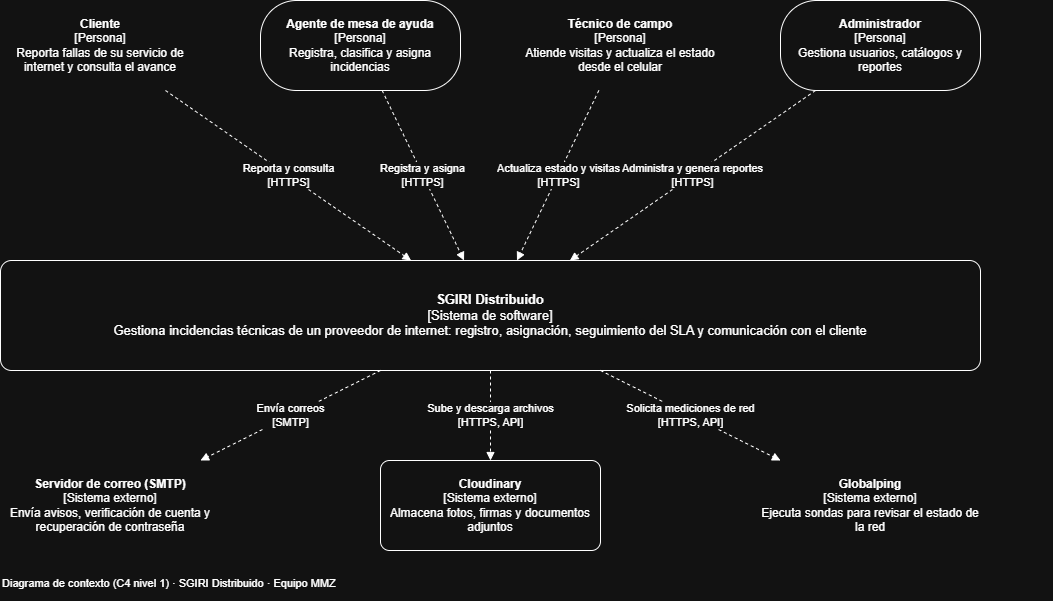
\includegraphics[width=\textwidth]{diagramas/C4-nivel-1-SGIRI.png}
\caption{Diagrama de contexto de SGIRI Distribuido (nivel 1 del modelo C4).}
\label{fig:c4n1}
\end{figure}

\subsection{Nivel 2: contenedores}

\begin{figure}[H]
\centering
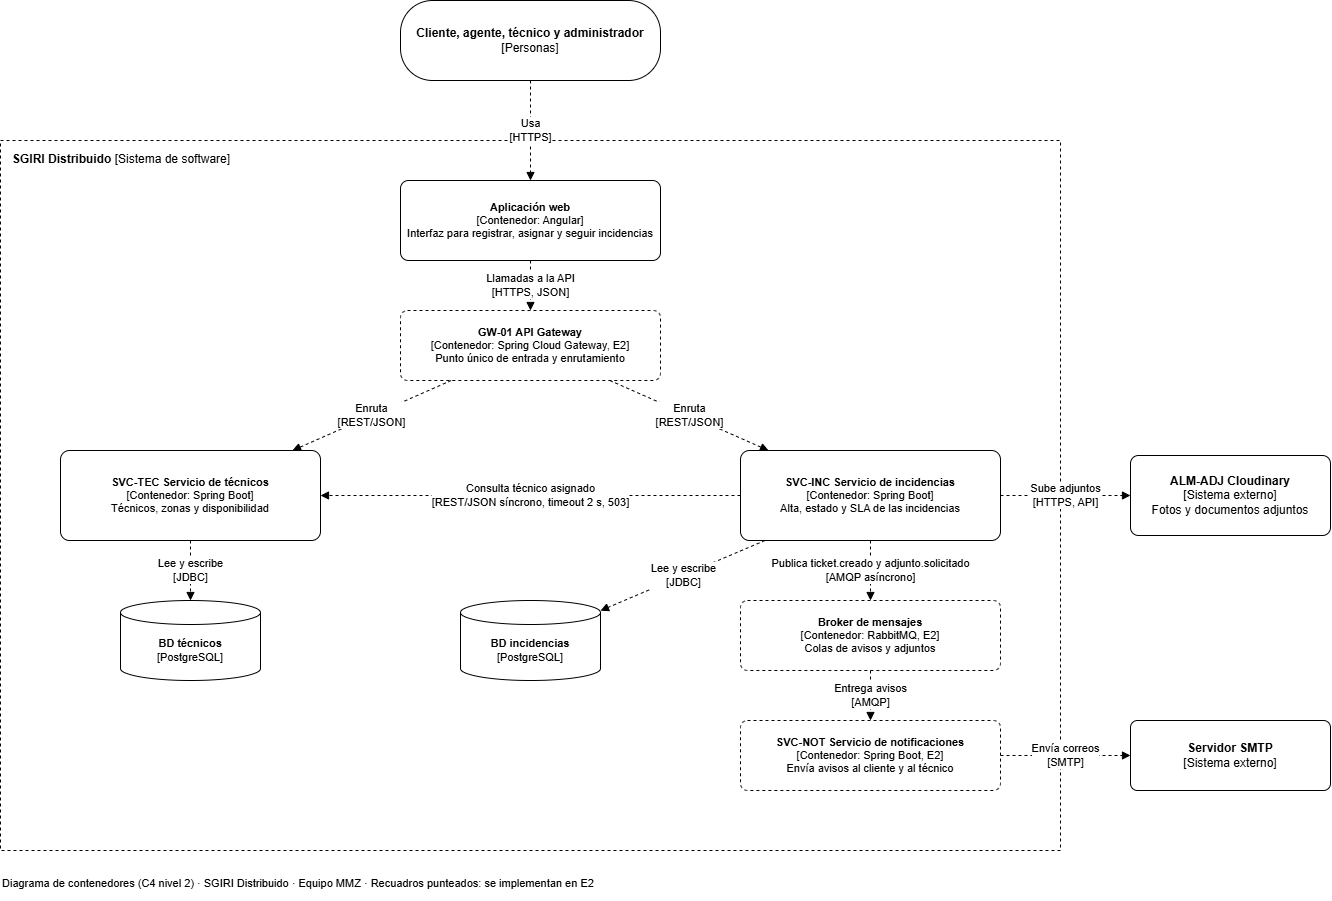
\includegraphics[width=\textwidth]{diagramas/C4-nivel-2-SGIRI.png}
\caption{Diagrama de contenedores: servicios, bases de datos y comunicación (nivel 2 del modelo C4).}
\label{fig:c4n2}
\end{figure}

\section{Modelo de comunicación entre servicios}
\label{sec:comunicacion}

Cada interacción del diagrama de contenedores se clasifica por tipo (sincrónica o asincrónica),
mecanismo (REST, gRPC, mensajería) y la razón por la que se eligió, apoyada en lo medido en PE-U1
y en lo decidido en el ADR-002. Los identificadores son los mismos del diagrama de contenedores:
\texttt{SVC-INC} (incidencias), \texttt{SVC-TEC} (técnicos), \texttt{SVC-NOT} (notificaciones),
\texttt{GW-01} (API Gateway) y \texttt{ALM-ADJ} (almacenamiento de adjuntos).

\begin{longtable}{@{}p{2.5cm} p{1.9cm} p{1.9cm} p{3.9cm} p{3.9cm}@{}}
\caption{Interacciones entre contenedores}
\label{tab:comunicacion}\\
\toprule
Interacción & Tipo & Mecanismo & Justificación & Tolerancia a fallos \\
\midrule
\endfirsthead
\toprule
Interacción & Tipo & Mecanismo & Justificación & Tolerancia a fallos \\
\midrule
\endhead
\bottomrule
\endfoot
\texttt{SVC-INC} $\rightarrow$ \texttt{SVC-TEC}
& Sincrónica & REST/JSON & El agente espera la respuesta para asignar; el dato cambia poco y se
consulta con frecuencia & \emph{Timeout} 2 s, 2 reintentos, \texttt{503} controlado \\
\addlinespace
\texttt{SVC-INC} $\rightarrow$ \texttt{SVC-NOT}
& Asincrónica & Mensajería (AMQP) & El aviso no debe bloquear el alta; si falla, se reintenta sin
perder el ticket & Cola con reintento y cola de fallos \\
\addlinespace
\texttt{SVC-INC} $\rightarrow$ \texttt{ALM-ADJ}
& Asincrónica & Mensajería (AMQP) & Mitiga el riesgo R-03: el ticket se registra primero y el
adjunto se sube después & Reintento con límite; estado «adjunto pendiente» \\
\addlinespace
Cliente $\rightarrow$ \texttt{GW-01} $\rightarrow$ servicios
& Sincrónica & REST/JSON & Punto único de entrada, autenticación y límites de tasa & Gateway con
verificación de salud \\
\end{longtable}

\section{Análisis CAP y PACELC}
\label{sec:cap}

El teorema CAP describe qué se sacrifica durante una partición de red~\cite{gilbert2012}; PACELC
agrega qué se sacrifica cuando no la hay~\cite{abadi2012}. La tabla se lee por dato crítico, no por
servicio.

\begin{longtable}{@{}p{3.3cm} p{4.3cm} p{3.9cm} p{3.5cm}@{}}
\caption{Decisión CAP/PACELC por dato crítico}
\label{tab:cap}\\
\toprule
Dato crítico & En partición (CAP) & Sin partición (PACELC) & Consecuencia para el usuario \\
\midrule
\endfirsthead
\toprule
Dato crítico & En partición (CAP) & Sin partición (PACELC) & Consecuencia para el usuario \\
\midrule
\endhead
\bottomrule
\endfoot
Estado del ticket & \textbf{CP}: se rechaza la escritura antes que aceptar un estado dudoso &
\textbf{EC}: se espera la confirmación antes de responder &
El técnico ve un error y reintenta; nunca ve un ticket «resuelto» que en realidad no lo está (RNF-02) \\
\addlinespace
Asignación al técnico & \textbf{CP}: no se asigna sin confirmación del servicio de técnicos &
\textbf{EC}: consistencia antes que latencia &
Si el servicio de técnicos no responde, el agente puede guardar el ticket como «sin asignar» y
asignarlo después; no se pierde el caso (RNF-02) \\
\addlinespace
Notificaciones y adjuntos & \textbf{AP}: se acepta el evento y se entrega cuando la red vuelva &
\textbf{EL}: latencia antes que consistencia &
El cliente recibe el aviso con retraso, pero el ticket ya existe (RNF-02, RNF-06) \\
\addlinespace
Consulta de disponibilidad de técnicos & \textbf{AP}: se responde con la última copia conocida &
\textbf{EL} &
El agente puede ver una disponibilidad desactualizada por segundos; el sistema lo advierte (RNF-03) \\
\addlinespace
Auditoría de cambios & \textbf{AP}: se registra localmente y se replica después &
\textbf{EL} &
Ninguna operación se pierde del registro aunque el nodo de auditoría esté caído (RNF-01) \\
\end{longtable}

\section{Registros de decisiones de arquitectura}

Los ADR completos están en \texttt{docs/adr/} y se versionan con el repositorio.

\begin{table}[H]
\centering
\caption{Resumen de los ADR}
\label{tab:adr}
\small
\begin{tabularx}{\linewidth}{@{}lYY@{}}
\toprule
ADR & Decisión & Consecuencia principal \\
\midrule
ADR-001 & Microservicios por dominio con API Gateway, sin orquestación compleja &
Despliegue independiente y aislamiento de fallos, a cambio de complejidad operativa que se acota a
cinco servicios \\
\addlinespace
ADR-002 & REST/JSON síncrono para consultas y mensajería asíncrona para notificaciones y adjuntos &
Consultas predecibles; el alta no depende de servicios externos \\
\bottomrule
\end{tabularx}
\end{table}

\section{Riesgos}
\label{sec:riesgos}

Los tres primeros riesgos provienen del análisis de FORM-AC-01 (incidente de Fastly del 8 de junio
de 2021, \cite{fastly2021}) aplicado a SGIRI; los dos restantes son propios de este proyecto.

\begin{longtable}{@{}p{0.8cm} p{4.6cm} p{1.0cm} p{1.1cm} p{5.9cm}@{}}
\caption{Riesgos técnicos, probabilidad, impacto y mitigación}
\label{tab:riesgos}\\
\toprule
ID & Riesgo & Prob. & Impacto & Medida de mitigación verificable \\
\midrule
\endfirsthead
\toprule
ID & Riesgo & Prob. & Impacto & Medida de mitigación verificable \\
\midrule
\endhead
\bottomrule
\endfoot
R-01 & Un cambio válido en las reglas de transición deja el ticket sin salida y con el SLA
corriendo & Media & Alto & Validar la máquina de estados; transición inválida devuelve \texttt{409}
sin alterar estado ni contador; pruebas de todas las transiciones \\
\addlinespace
R-02 & Un despliegue con credencial o URL mal configurada no arranca y, con una sola instancia,
detiene todo el servicio & Media & Muy alto & Dos instancias con verificación de salud antes de
recibir tráfico; conservar artefacto anterior; arranque verificado en entorno de prueba \\
\addlinespace
R-03 & El alta de la incidencia depende de un servicio externo de adjuntos y termina en error 500 &
Alta & Alto & Registrar el ticket primero y subir después, con tiempo límite y reintento; prueba con
el servicio externo bloqueado \\
\addlinespace
R-04 & \pendiente{riesgo propio: por ejemplo, coherencia de datos entre el ticket y el técnico
asignado} & \pd & \pd & \pendiente{} \\
\addlinespace
R-05 & \pendiente{riesgo propio: por ejemplo, dependencia de la conectividad del local del cliente}
& \pd & \pd & \pendiente{} \\
\end{longtable}

\section{Plan del proyecto}

\subsection{Roles y responsabilidades}

\begin{table}[H]
\centering
\caption{Roles del equipo y entregables de cada uno}
\label{tab:roles}
\small
\begin{tabularx}{\linewidth}{@{}lYY@{}}
\toprule
Integrante & Rol y responsabilidad & Entregables \\
\midrule
Zambrano Yong Angel Daniel & Arquitecto y Responsable de Documentación & Diagramas C4, ADR-001 y
ADR-002, modelo de comunicación, CAP/PACELC, justificación distribuida, integración del documento,
tablero y bitácora \\
\addlinespace
Mendoza Bermello Angello Agustín & Líder de Desarrollo & Esqueleto en \texttt{src/}, comunicación
entre servicios, instrucciones de ejecución, capturas \\
\addlinespace
Macías Vásquez César Abraham & Responsable de Calidad & Historias de usuario, RNF con ISO/IEC 25010,
riesgos, trabajos relacionados, pruebas y revisión de coherencia \\
\bottomrule
\end{tabularx}
\end{table}

En un equipo de tres integrantes, el Arquitecto asume además el rol de Responsable de
Documentación.

\subsection{Cronograma de las cuatro entregas}

\begin{table}[H]
\centering
\caption{Cronograma alineado con el calendario del encuadre}
\label{tab:cronograma}
\small
\begin{tabularx}{\linewidth}{@{}llY@{}}
\toprule
Entrega & Semana & Contenido comprometido \\
\midrule
E1 & 5 (23 al 29 de noviembre de 2026) & Definición, requisitos, arquitectura C4, ADR, CAP/PACELC,
esqueleto de dos servicios \\
\addlinespace
E2 & 9 & Microservicios completos, API documentada, contenedores \\
\addlinespace
E3 & 13 & Base de datos distribuida y procesamiento de datos del SLA \\
\addlinespace
E4 & 17 & Sistema final en capas, calidad, pruebas y defensa \\
\bottomrule
\end{tabularx}
\end{table}

\subsection{Tablero de trabajo y tareas}

Las tareas se gestionan como \emph{issues} en GitHub Projects, con un issue por entregable, un
responsable y un criterio de aceptación. Los issues de E1 y de E2 quedan asignados desde la primera
semana, de modo que la segunda entrega no empieza de cero.

\begin{table}[H]
\centering
\caption{Tareas de E1 y E2 y su responsable}
\label{tab:tareas}
\small
\begin{tabularx}{\linewidth}{@{}lYl@{}}
\toprule
Entrega & Tarea & Responsable \\
\midrule
E1 & Estructura del repositorio, README, bitácora y tablero & Angel \\
E1 & Diagrama C4 nivel 1 y ADR-001 & Angel \\
E1 & Diagrama C4 nivel 2, ADR-002 y tabla de comunicación & Angel \\
E1 & Justificación distribuida y análisis CAP/PACELC & Angel \\
E1 & Esqueleto: servicio de técnicos & Angello \\
E1 & Esqueleto: servicio de incidencias y comunicación entre ambos & Angello \\
E1 & Instrucciones de ejecución y capturas & Angello \\
E1 & Historias de usuario con criterios de aceptación & César \\
E1 & Requisitos no funcionales con cifras e ISO/IEC 25010 & César \\
E1 & Análisis de riesgos y trabajos relacionados & César \\
E1 & Revisión de coherencia y pruebas del esqueleto & César \\
E1 & Documento integrado, video y PDF del SGA & Todo el equipo \\
E2 & Contenedores y API Gateway & Angello \\
E2 & Contratos OpenAPI versionados & César \\
E2 & Despliegue en contenedores y pruebas de humo & Angel \\
\bottomrule
\end{tabularx}
\end{table}

\subsection{Reglas de trabajo}

\begin{enumerate}
\item Una rama por tarea y \emph{pull request} a \texttt{main}, aunque la revisión la haga otro
integrante del equipo.
\item Cada integrante confirma con su propia cuenta; ningún integrante sube trabajo de otro.
\item Una entrada en \texttt{BITACORA.md} por sesión, escrita el mismo día.
\item Toda decisión de arquitectura se registra como ADR antes de implementarse.
\item Antes de cada integración: \texttt{git pull --rebase} y compilación del documento.
\end{enumerate}

\section{Esqueleto funcional}

\subsection{Qué demuestra el esqueleto}

El esqueleto no implementa la lógica de negocio: demuestra que la base técnica distribuida
funciona. Dos servicios independientes, cada uno en su proceso y su puerto, se comunican por el
mecanismo elegido en el ADR-002: el servicio de incidencias consulta al de técnicos y devuelve la
respuesta combinada.

\begin{table}[H]
\centering
\caption{Componentes del esqueleto}
\label{tab:esqueleto}
\small
\begin{tabularx}{\linewidth}{@{}lllY@{}}
\toprule
Servicio & Puerto & Rol & Endpoint demostrativo \\
\midrule
\texttt{servicio-tecnicos} & 8081 & Proveedor & \texttt{GET /api/tecnicos}, \texttt{GET /api/tecnicos/\{id\}},
\texttt{GET /actuator/health} \\
\addlinespace
\texttt{servicio-incidencias} & 8082 & Consumidor & \texttt{GET /api/incidencias/\{id\}} (resuelve el
técnico llamando al puerto 8081) \\
\bottomrule
\end{tabularx}
\end{table}

\subsection{Ejecución}

Las instrucciones completas están en el \texttt{README.md} de la raíz; en resumen, desde una
terminal por servicio:

\begin{verbatim}
cd src/servicio_tecnicos    && python app.py    # http://localhost:8081
cd src/servicio_incidencias && python app.py    # http://localhost:8082
curl -i http://localhost:8082/api/incidencias/1
\end{verbatim}

\pendiente{Agregar aquí la salida real de la verificación, con fecha de la ejecución.}

\subsection{Evidencia de ejecución}

\begin{figure}[H]
\centering
\figurapendiente{Captura 1: ambos servicios en marcha, con usuario, máquina, fecha y hora visibles}
\caption{Esqueleto en ejecución: servicios activos y llamada entre ellos.}
\label{fig:captura1}
\end{figure}

\begin{figure}[H]
\centering
\figurapendiente{Captura 2: respuesta combinada del consumidor con los datos del proveedor}
\caption{Respuesta del servicio de incidencias con datos resueltos del servicio de técnicos.}
\label{fig:captura2}
\end{figure}

\begin{figure}[H]
\centering
\figurapendiente{Captura 3: degradación controlada con el proveedor detenido (503, no 500)}
\caption{Comportamiento ante la caída del servicio proveedor: degradación controlada.}
\label{fig:captura3}
\end{figure}

\section{Aportes del equipo}

Los enlaces apuntan a las confirmaciones y a los issues reales; la tabla se actualiza el último día
con los números definitivos.

\begin{table}[H]
\centering
\caption{Aportes por integrante}
\label{tab:aportes}
\small
\begin{tabularx}{\linewidth}{@{}lYl@{}}
\toprule
Integrante & Aporte principal & Enlaces \\
\midrule
Angel (\texttt{@iMouraad}) & Arquitectura, ADR, C4, CAP/PACELC, documento & \pendiente{commits e issues} \\
Angello (\texttt{@Amendozab5}) & Esqueleto, comunicación, ejecución, capturas & \pendiente{commits e issues} \\
César (\texttt{@CesarMacias007}) & Requisitos, riesgos, pruebas, coherencia & \pendiente{commits e issues} \\
\bottomrule
\end{tabularx}
\end{table}

\section{Declaración de uso de inteligencia artificial}

\pendiente{Completar con la verdad, herramienta por herramienta. Formato sugerido:}

\begin{table}[H]
\centering
\caption{Uso de herramientas de inteligencia artificial}
\small
\begin{tabularx}{\linewidth}{@{}llYY@{}}
\toprule
Herramienta y versión & Para qué se usó & Qué se verificó & Cómo se verificó \\
\midrule
\pendiente{} & \pendiente{} & \pendiente{} & \pendiente{} \\
\bottomrule
\end{tabularx}
\end{table}

% ---------------------------------------------------------------------
% Si no se usó IA, se escribe una sola frase indicándolo y se elimina
% la tabla. Si se usó, se declara también lo usado en los documentos
% previos (FORM-AC-01 declaró ChatGPT y Claude). No declararlo es un
% problema de integridad, no de estilo.
% ---------------------------------------------------------------------


% ---------------------------------------------------------------------
% Referencias
% ---------------------------------------------------------------------
\clearpage
\printbibliography[heading=bibintoc,title={Referencias}]

% ---------------------------------------------------------------------
% Anexos
% ---------------------------------------------------------------------
\appendix
\section{Trazabilidad entre el levantamiento y el diseño}
\label{anexo:trazabilidad}

Esta tabla es la que permite comprobar, sin leer todo el documento, que cada requisito nace de algo
que el entrevistado dijo y que cada requisito tiene un lugar en la arquitectura.

\begin{table}[H]
\centering
\caption{Trazabilidad: pregunta del guion $\rightarrow$ requisito $\rightarrow$ contenedor}
\label{tab:trazabilidad}
\small
\begin{tabularx}{\linewidth}{@{}llYl@{}}
\toprule
Pregunta del guion & Requisito & Decisión de arquitectura que lo atiende & Contenedor \\
\midrule
Guion, P5 (sin validar) & RF-01 & Alta rápida y persistencia desacoplada del adjunto (ADR-002) & \texttt{SVC-INC} \\
\addlinespace
Guion, P6 (sin validar) & RF-02, RF-03 & Consulta y asignación de técnicos con balanceo de carga & \texttt{SVC-TEC} \\
\addlinespace
Guion, P10, P12 (sin validar) & RNF-01 & Réplicas por servicio con verificación de salud y RTO $<$ 30 min (ADR-001) & \texttt{GW-01} \\
\addlinespace
FORM-AC-01 (R-03) & RNF-02 & Mensajería asíncrona para adjuntos; respuesta \texttt{503} si proveedor falla & \texttt{SVC-INC}, cola \\
\addlinespace
FORM-AC-01 (R-01) & RF-11 / R-01 & Validación estricta de máquina de estados con \texttt{409 Conflict} & \texttt{SVC-INC} \\
\bottomrule
\end{tabularx}
\end{table}

\section{Acta de levantamiento de información}
\label{anexo:acta}

La entrevista con el proveedor de internet no se realizó antes del cierre de E1, porque el
entrevistado no estuvo disponible. Por eso no hay acta firmada ni grabación. Los requisitos citan
la pregunta del guion (\texttt{docs/levantamiento/guion-entrevista.md}) de la que se espera
obtener el dato, marcada como \emph{sin validar}, y las cifras de la línea base quedan pendientes.
La entrevista se hará antes de E2; con sus respuestas se ajustarán los requisitos y esta tabla.

\section{Verificación de referencias}

\begin{table}[H]
\centering
\caption{Comprobación de cada referencia}
\small
\begin{tabularx}{\linewidth}{@{}lYl@{}}
\toprule
Clave & Comprobación realizada & Fecha \\
\midrule
\texttt{li2022incident} & DOI (\url{https://doi.org/10.1145/3544497.3544499}) abre la obra correcta en ACM Digital Library y los datos bibliográficos coinciden con Crossref. & 22/11/2026 \\
\addlinespace
\texttt{harsh2023murphy} & DOI (\url{https://doi.org/10.1145/3603269.3604877}) abre la obra correcta en ACM SIGCOMM y metadatos verificados en Crossref. & 22/11/2026 \\
\addlinespace
\texttt{li2023identifying} & DOI (\url{https://doi.org/10.1109/ISSRE59848.2023.00028}) abre la publicación de IEEE ISSRE y metadatos verificados en Crossref. & 22/11/2026 \\
\addlinespace
\texttt{gilbert2012} & DOI (\url{https://doi.org/10.1109/MC.2011.389}) comprobado en IEEE Computer Society y verificado en Crossref. & 22/11/2026 \\
\addlinespace
\texttt{abadi2012} & DOI (\url{https://doi.org/10.1109/MC.2012.33}) comprobado en IEEE Computer Society y verificado en Crossref. & 22/11/2026 \\
\addlinespace
\texttt{basiri2016} & DOI (\url{https://doi.org/10.1109/MS.2016.60}) comprobado en IEEE Software y verificado en Crossref. & 22/11/2026 \\
\bottomrule
\end{tabularx}
\end{table}


\end{document}
